\part{文字与段落}
这里首先要明确一下再latex中的各类长度单位,具体如下所示:
\begin{figure}[H]
	\centering
	\begin{tabular}{cl}
		\hline
		pt & 点阵宽度,1/72.27in \\
		bp & 点阵宽度,1/72in \\
		in & 点寸 \\
		cm & 厘米 \\
		mm & 毫米 \\
		\hline
		em & 当前字号下大写字母M的宽度,常用于水平距离的设定\\
		ex & 当前字号下小写字母m的高度,常用于垂直距离的设定\\
		\hline
	\end{tabular}
\end{figure}
\section{全局字体类型设置}
\begin{lstlisting}[style = LaTeX_TeXworks]
\usepackage{fontspec}							% 自定义字体宏包

% 中文字体设置
\setCJKfamilyfont{Songti}{宋体}				   % 导入本地宋体字体
\setCJKfamilyfont{Kaiti}{楷体}				   % 导入本地楷体字体
\setCJKfamilyfont{Heiti}{黑体}				   % 导入本地楷体字体
\newcommand{\Song}{\CJKfamily{Songti}}			% 设置\Song为宋体的指令,方便下文的局部使用	
\newcommand{\Kai}{\CJKfamily{Kaiti}}			% 设置\Kai为楷体的指令,方便下文的局部使用
\newcommand{\Hei}{\CJKfamily{Heiti}}			% 设置\Hei为黑体的指令,方便下文的局部使用
\setCJKmainfont{宋体}							   % 设置全局默认字体为宋体

% 英文字体设置
\newfontfamily{\TimesNewRoman}{Times New Roman}	% 导入本地Times New Roman字体
\setmainfont{Times New Roman}					% 设置全局

% 设置一个字体复位的命令
\newcommand\resetfont{\Song \TimesNewRoman}		% 方便字体变更后一键复位
\end{lstlisting}
\section{全局字号设置}
\begin{lstlisting}[style = LaTeX_TeXworks,numbers=none]
\documentclass[12pt]{article}				% 全局字体为12榜,即小四号字体
\end{lstlisting}
\begin{figure}[H]
	\centering
	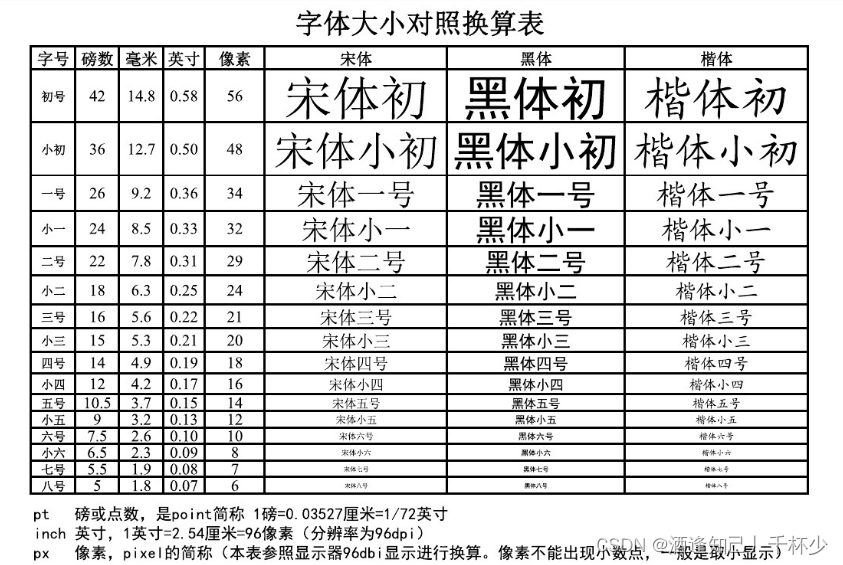
\includegraphics[height = 10cm, width = 15cm]{figure/字号对照表.png}		% 插入本地图片
\end{figure}
\section{全局段落格式设置}
\begin{lstlisting}[style = LaTeX_TeXworks]
\usepackage{indentfirst}							% 加载 indentfirst 宏包,用于使得文档中所有章节后的第一个段落也进行缩进。
\setlength{\parindent}{2em}							% 设置段落的缩进为 2em,即段落开头缩进 2 个字符宽度。
\setlength{\leftskip}{1em}							% 将段落左侧的距离设置为 1em
\setlength{\rightskip}{1em}							% 将段落右侧的距离设置为 1em
\setlength{\parskip}{1ex plus 0.5ex minus 0.2ex}	% 设置段落之间的垂直距离为 1ex,允许在需要时拉伸至多 0.5ex 或压缩至多 0.2ex
\fontsize{12}{14}									% 一个设置字号和行间距的命令(但是一般不使用)
\linespread{1.25}									% 将行距设置为当前字号的 1.25 倍。
\end{lstlisting}
这个地方需要注意的是\addbs{linespread}命令,他后面的参数是基础行距的倍数,而基础行距在不使用\addbs{fontsize}指令更改的情况下即为当前字号的大小。
\section{局部设置}
\begin{lstlisting}[style = LaTeX_TeXworks]
\noindent{无首行缩进的一段}
{\linespread{2.0}\selectfont 两倍行间距的一段\par}
\vspace{6pt}			% 插入垂直间距
\hspace{6pt}			% 插入水平间距
{\SinSun \zihao{-4} 小四宋体的字体\par}
\textbf{这段文字将被加粗}
\textit{这段文字将倾斜}
\usepackage{ulem}
\uline{这段文字将加入下划线}
\end{lstlisting}
\section{换行操作}
在\LaTeX 中,常见的换行操作有4种:
\begin{enumerate}
	\item
	\textbackslash\textbackslash 和\addbs{newline}实现段内换行
	\item
	一行空行和\addbs{par}实现段落的切换 
\end{enumerate}
\section{对齐方式}
\begin{enumerate}
	\item
	\addbs{raggedright} :左对齐
	\item
	\addbs{raggedleft}:右对齐
	\item
	\addbs{centering}:居中 
\end{enumerate}

